\documentclass[a4paper]{article}
\usepackage{graphicx}

\begin{document}

{\Large{The present-day unharmonic changes are directed differently in the divided kingdom of eukaryotes}}

{ \small{... never send to know for whom the bell tolls...} }

Sergey Feranchuk \\{\small(self-employed; residence: Smolensk, Russia; e-mail: feranchuk@gmail.com)}

\begin{flushright}
\small{ \textit{to my mother}}
\end{flushright}

\section*{Abstract}

%Речь в работе идет о соотношении периодических ритмов с нерегулярными. Более узко, для микро-экосистем почвы, периодические пожары приводят к обновлению экосистем, как и намеренное регулярное освобождение от посевов, для  сельскохозяйстенных земель. Образцы почвы, и из человека - посмотрели состав микроорганизмов. Смотрели "по крупному", обзорно.

%В таком взгляде много общего, между разными сообществами микроорганизмов. То что бы можно было тут увидеть - признаки нестабильности, скрытой накопившейся нестабильности вследствии изменений режима периодичных воздействий на микро-сообщества в последние десятиления.
\clearpage

\section*{Introduction}

Harmonic oscillator is a simplest mathematical model which can simulate periodic changes as a physical phenomenon. It is exactly solvable both in classical and in quantum physics. The simplest extension of harmonic oscillator model is to introduce a quadratic term to the linear equation of the model. 

The changes in the surrounding nature are often distinguish from a harmonic periodicity. The marginal cases of unharmonicity are a chaotic noise and an abrupt crash. Attempts to manage these extreme cases by means of ''traditional'' science are knowingly wrong, although some empirical rules do observed in these processes.

Suitable for a minimally simple approach to systematically describe in some way the possible distortions of a periodicity is the model of harmonic oscillator with an introduced perturbation, like the unharmonic oscillator model mentioned above. 

The problem in any crash is to be ready for it, and the prediction of crash is impossible. As in the cases of a phase transition, the mixing of large-scaled and local-scale factors occurs and is of importance in a transitional period. Anyway any clever decisions in a crisis time are always based on a rational reasoning even if this reasoning do not fit to a format of a ''traditional'' science which has been developed for another purposes.

As an attempt to rationally describe the risks which are accumulated in microbial communities at resent times, a wide and broad look is proposed here to a composition of some selected communities. The simple model of unharmonic oscillations can be of use to measure and clarify in some way an unharmonicity in the composition of the communities.

Recent advances in sequencing technologies lead to the ''outbreak'' in the microbiology. A wide classes and even kingdoms of poorly known living creatures become visible in the common and custom microbiological samples. The present research is focused on eukariotic part of the microbiomes for the purposes declared in it. Besides the kingdoms of animals, plants and fungi, it is presently extended to include much of another eukariotic species, mostly unicellular, hardly classified and poorly investigated. Some of them are supposed to be conservative and neutral, some are highly adaptive and predator-oriented. The group of eukariotic divisions known as SAR (''\textit{Strametopiles}'',''\textit{Alveolata}'',''\textit{Cercozoa}'') was introduced to broadly join the species with the latter of the strategies. These divisions are considered separately and other unicellular divisions with mostly first of the strategies are joined together in the analysis provided below.


\section*{Methods} 

%Для минимально простого описания искажений периодичности, подойдет модель осциллятора с малым дополнением, внесенным в закон движения, так что в колебаниях такого ''не-гармонического'' осциллятора проявляются отклонения от гармонического закона - то что может являеться признаком потенциальной неустойчивости.

A solution of quantum harmonic oscillator model is a uniform series of energy levels. An unharmonicity to that model is introduced by adding an extra perturbation so that a hamiltonian function for this model becomes to be $\hat H = p^2 + x^2 + \lambda x^4$. Here, $\lambda$ is a value of the non-linear perturbation. A ''clasical'' equation of motion for this oscillator, $\frac{dx}{dt} = -p; \frac{dp}{dt} = -x -\lambda x^3$. In the solutions of this equation, a positive perturbation increases oscillation frequency (fig 1). In the quantum model, energy levels of the perturbed oscillator become to be distributed not uniformly [1]. So, the unharmonic perturbation is differ from just an increase of oscillation frequency. The qualitative difference depends on a direction of unharmonicity. Positive perturbation increases frequency of higher garmonics and in a marginal case lead to an instability and a sudden crash, as it is by another means is approached in the extensions of the fractal theory [2]. Negative perturbation in another marginal case means a transformation of the potential surface, up to a possibility of quantum transitions beyond its bounds and a disappearnce of the oscillations.  

The so-called ''rank-abundance charts'' in ecology allow to reveal specific features of a particular ecosystem. Varioius models are proposed to describe it and any of the models do not cover all of the cases of ecosystems. The so-caled ''Zipf-Pareto'' distribution and the Boltzmann distribution are among the most suitable models in a generic case, as it was discussed in [3]. Boltzmann distribution is applicable in full to some another classes of systems, like an ideal gas, and so is Zipf-Pareto distribution, for the e.g. income in a society. In these systems Boltzman distribution binds the linear increase of energy from level to level and exponential decrease of population in an energy level; the same is for a Zipf-Pareto distribution although the ''energy'' there is implicit and is expressed from the observable values by a logarithmic law. If the distribution of energy levels is changed it should be seen in a shape of rank-abundance charts, in the frames of the both models. This way the influence of the direction of unharmonicity introduced above to the change of shape of a rank-abundance charts is schematically drawn in figure 1.

For the purposes of analysis, were used, selectively, samples from the experiments where the genetic material of microbial communities was sequenced; these experiments were conducted by different scientific groups in different time and by different reasons. Archives of DNA fragments were obtained from public repositories.  

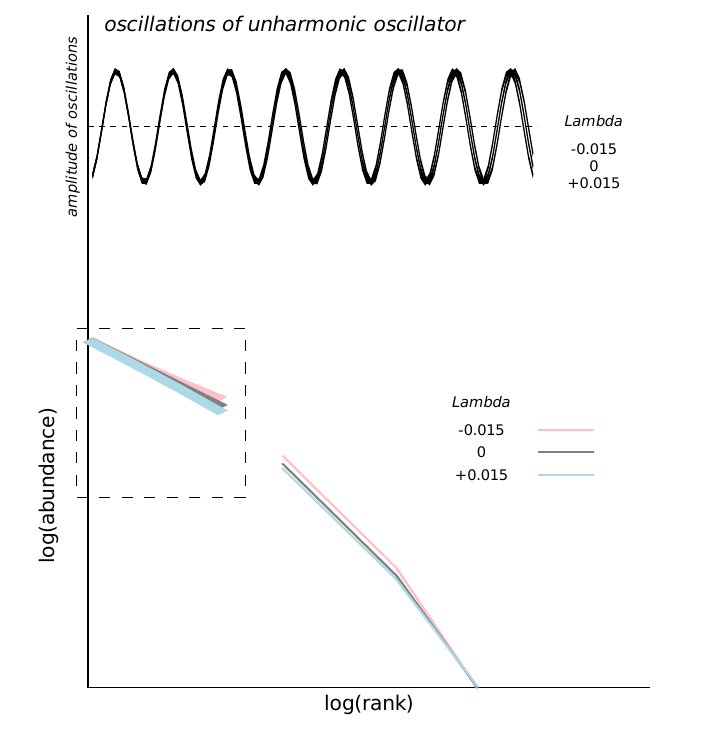
\includegraphics[width=0.92\textwidth]{rankabundance_unharmonic.jpg}

Figure 1 \textit{Bias of oscillation frequency and bias of abundance distributions, in Zipf-Pareto model (in the frame) and in Boltzman model, for differtend signs of $\lambda$ in unharmonic oscillator}


\section*{Results} 


All six of the processed samples were joined together to get the rank-abundance charts of a broad scope. The resulted charts for the five broad divisions of eukaryotes are shown in fig 2A. Following the definition, the relative quantities of the most abundant species are in the left part of the chart, and of the minor species - in the right part. The differences between eukaryotic divisions which are seen in these charts is better to express in terms of ''rich'' and ''poor'' classes within a division. For animals, both frequent and rare species are vulnerable to instability ended by a sudden crash. For plants, the less abundant and minor species are in the opposite side and are expected to be winners in the approaching crisis. For the kingdom of fungi the rare species are instead unstable and vulnerable, and the dominant species are kept strong.   

The lesser is known about various groups of unicellular species which are considered in the frames of the introduced approximated division. It can be seen anyway that rare and minor species from the SAR group are kept as stable as rare plants. The relative composition of the divisions in each of the analyzed samples is provided in fig 2B. The range of samples is from soil in England in 2002 up to the soil in the Middle East desert in 2018. Although the heterogeneity of the selected samples is reflected in full in the presented diagrams, the trend for a relative increase of SAR division in recent times can be noticed. Another groups of unicellular species which are assumed to be at most conservative and neutral are in middle-point position in the rank-abundance chart declining to neither of sides in the expected crisis; and their relative presence is reduced in some samples closer to the recent years.

The yeast are abundant in the group of fungi, although it can be in part caused by biases in the reference database of representative eukaryotic rRNA sequences. Some of them are known to be pathogenic for humans, like the species of Candida genera; some another also can expected to have a pathogenic strategy. Also in the chart in fig 2B in separate bars in red are shown another groups of species which can be danger pathogens of humans. These are, \textit{Nematoda} worms in samples 1 and 6, \textit{Platyhelmintes} in sample 4,  traces of \textit{Microsporidia} species are in samples 1 and 2, \textit{Apicomplexa} in sample 1, \textit{Haplosporida} and traces of \textit{Cnidaria} in sample 6.


\newpage

{\large{\textbf{A}}}\\
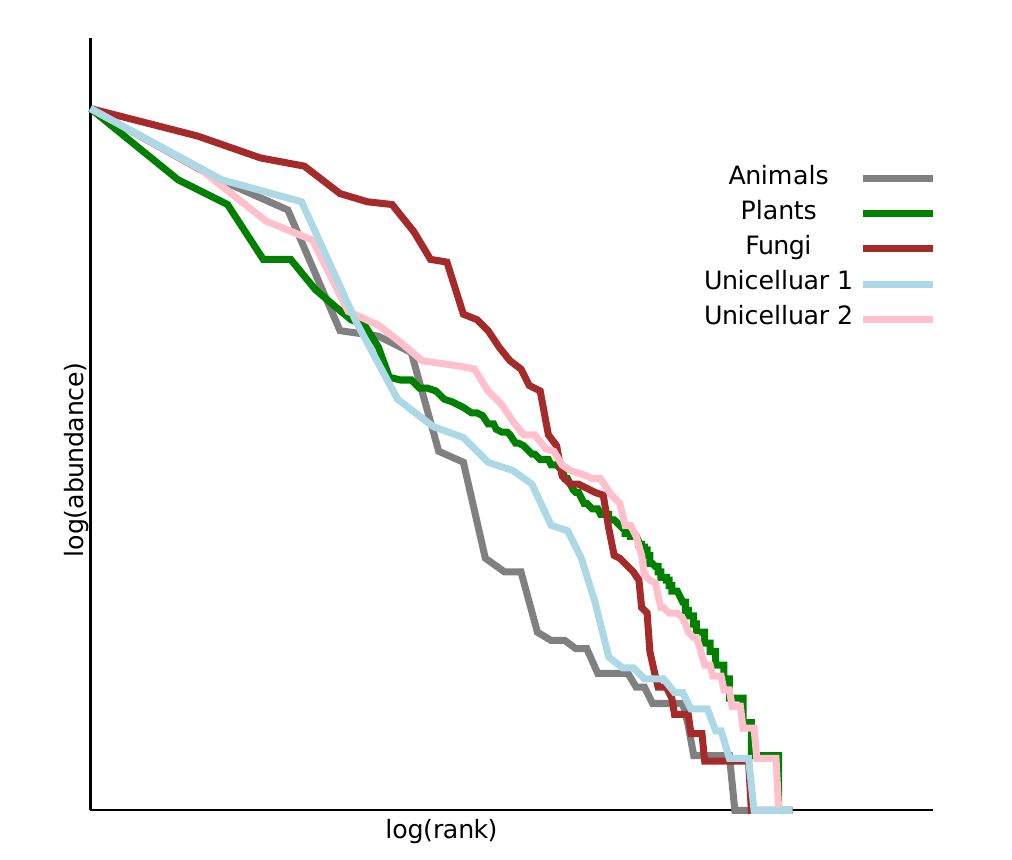
\includegraphics[width=0.92\textwidth]{rankabundance.jpg}\\
{\large{\textbf{B}}}\\
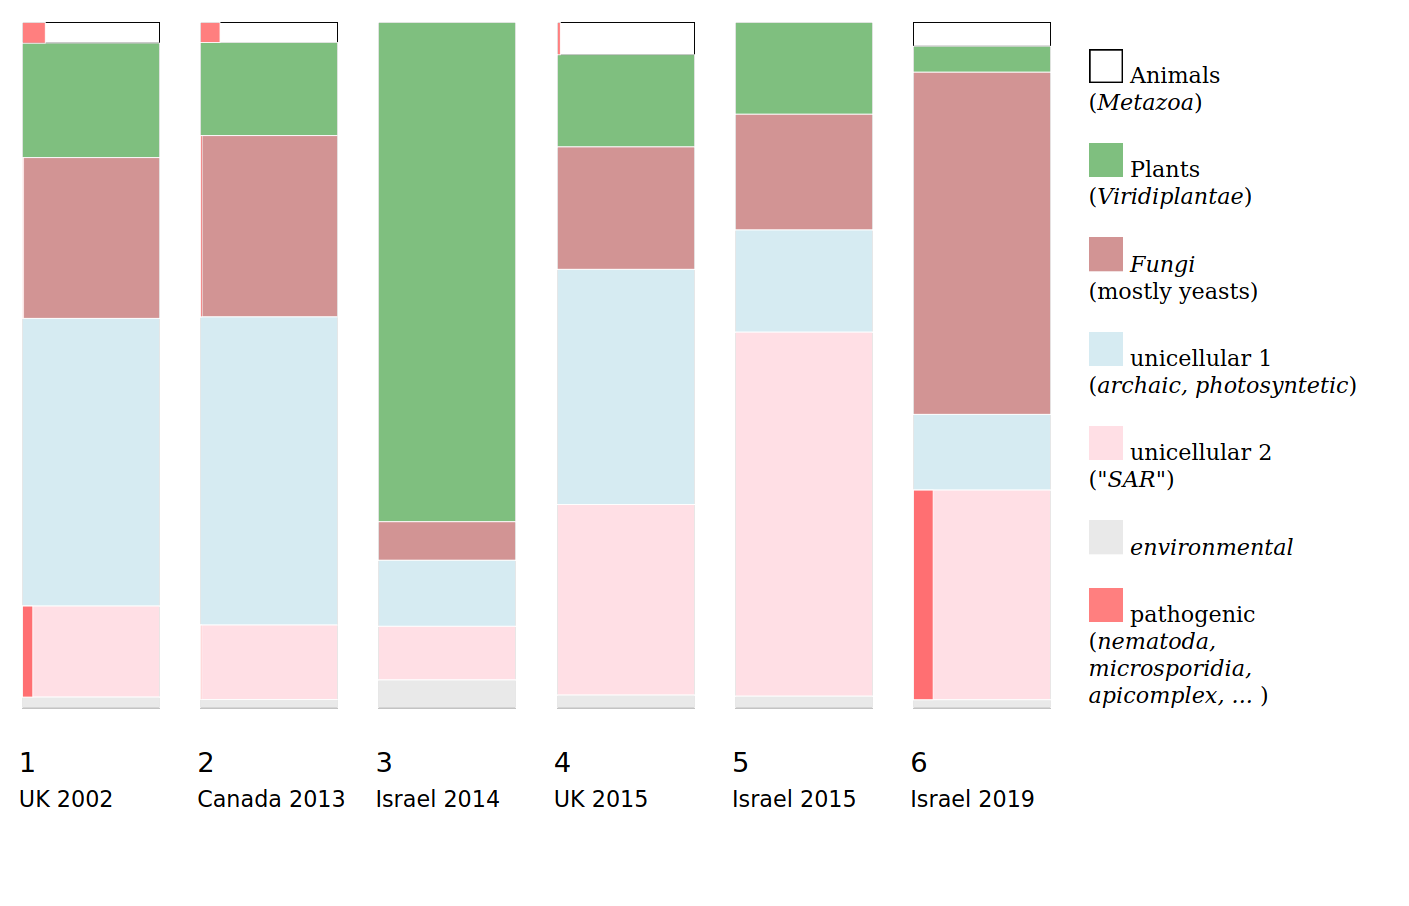
\includegraphics[width=0.92\textwidth]{tilechart.jpg}\\

Figure 2 \textit{(A) Rank-abundance charts for separated kingdoms of eukaryots.}
\textit{(B) Relative composition of samples, shown in separate columns.}




%Сводя вопрос сравнения численности видов к сравнению неустойчивости групп при сменах времен года, месяцев, дней и ночей, сменах дождей и яснй погоды, сменах полноводных паводков на маловодные при разливах рек - то что и определяет избыток питания в экологических нишах и под-группах, и ''заселенность'' в этих нишах - признаки искажения такой периодичности, индуцируимые через обратную связь, были бы признаком неусточивости.

%Не говоря о разнообразных группах одноклеточных организмов, про которые мало известно, для трех царст живого направления их отклонения, по диаграммам численности, показны ниже:


\section*{Discussion}


The periodic change of seasons, or an occasional burning of forests are adopted and accepted in a stable ecosystem. The fields were by a tradition were kept free from sowing to restore natural microbial balance in a soil. In the long enough period this tradition was kept out in most of agricultural lands. The hidden instability of microbial communities should anyway be anyway accumulated during this period. Microbes are extensively interchanged in the environment, the same species can be found in a soil, in human lungs or in gut. It can adopt to changes of the environment more flexibly than multicellular species, in favor to their own extensive reproduction.

All the above is a reason to draw the most precise attention to the properties of microbial communities which are symbiotic to humans or close enough to them. Although the events of the expected crisis are neither predicted nor described in the proposed model, the volume of data which was accumulated in recent years due to the outbreak in microbiology should be a subject of some large-scaled analysis. 

%Само событие кризиса в этой модели не описывается и не предсказывается. Эмпирически, колебания с нарастающим периодом - это признак риска кризиса [3]. В рамках самой модели квантового ангармонического осциллятора, ''сбой'' его движения возможен при отрицательном $\lambda$, через тоннельный переход в один из двух сегментов с отрицательной энергией за пределами области колебаний.

%\subsection*{Паразитические и патогенные виды - индикатор неусточивосчти?}

%На рисунке выделены красным группы, включающие паразитические организмы, потенциально вызывающие хронические трудно излечимые расстройства здоровья. Это, в образцах 



%''прорыв'' в микробиологии позволил увидеть больше в том что относися к микроорганизмам, акценты в описаниии причин и следствий привычных явлений в этом свете другие. в микробных сообществах есть общее, прагматически, микроорганизмы с земли, микроорганизмы с растений и животных переносятся легко и адаптируются быстрее чем ''хозяева''. что касается ''пахотного цикла'', эффект от его прекращения и сокращения, сказался бы на том общем, что есть во всех вышеупомянутых типах сообществ. долгосрочное накопление напряжения такого рода, как ожидается по постановке вопроса, как и любое накопление напряжения, имеет следствием риск ''взрыва'', ''обвала'', крупномасштабного кризиса.  


\section*{Conclusions}

The mixing of scales is an attribute of any crisis. Although the so-called fractal theory do utilize in some way the transformation of scales, it continue to be just empirical and incomplete couple of methods. The question continues to be opened and any other rational approaches to discover it are acceptable accordingly to a meaningful of obtained results.

Here, in a broad analysis of microbial communities, is is concluded that some instability can be detected in it, and most abundant species of yeast do contribute to an increase of this instability. The way to avoid any crisis is to keep a balance between a direction toward sudden crash and a direction towards fatal slow disappearance. Some of the divisions of the unicellular species are most close to this middle balance. The relative presence of these species is shortened in some samples closer to the recent years.


%В арсенале науки нет инструметов, чтобы с достоверностью обнаржить и проанализировать ход событий в переходный к кризисному период. Теория фракталов - один из методов, который применим к таким явлениям, как эмпирическое описание с заведомо мало-достоверным результатом.  Вопрос заведомо остается открытым и любые другие рациональные методы его исследовать приемлем, соразмерно с осмысленнстью полученных результатов.


\section*{References}

\begin{enumerate}

\item Feranchuk, I., Komarov, L., et al., Operator method in the problem of quantum unharmonic oscillator, Annals of Phys., 1995 

\item Nottale, L., Scale relativity and fractal space-time: theory and applications, arxiv.org, 2008

\item Feranchuk, S., Belkova, N., et al., Evaluating the use of diversity indices to distinguish between microbial communities with different traits. Res. Microbiol., 2018

\end{enumerate}

\newpage
\section*{Appendix A}

\textit{Formal specifications.}

\vskip 5pt

Listing of the samples used in the study.

\vskip 5pt

\begin{tabular}{lllllllll}
\hline
&Sample ID&Bases&Reads&Location&Date&18S RRNAs\\
\hline
1&ERR981203&5.3G&10M&51.83N 0.21E&2002.06.23&1517(*)\\
2&SRR6030929&2.4G&6.1M&42.98N 81.24W&2013&125002(*)\\
3&ERR588716&8.2M&159K&Israel&2014 or earlier&848\\
4&ERR970400&4.2G&13M&51.61N 3.95E&2015.01.01&18747 (*)\\
5&SRR7642476&77M&128K&30.78N 34.76E&2015.08.20&4231\\
6&SRR12806764&48M&97K&31.86N 34.72E&2019.02.25&116666\\
\hline
\end{tabular}

{\small(*) Volume of data was truncated.}

\vskip 5pt

Composition of the eukaryotic kingdoms.

\vskip 5pt

\begin{tabular}{ll}
\hline
Animals&\textit{Mollusca,Arthopoda}(*)\\
Plants&\textit{Chlorophyta,Streptophyta}\\
Fungi&\textit{Saccharomycotina} (*)\\
Unicellular 1&\textit{Euglenozoa,Rhodophyta,Haptophyta,Glaucophyta,Cryptophyta}\\
Unicellular 2&\textit{Cercozoa,Strametopiles,Alveolata,Acanthamoeba}\\
\hline
\end{tabular}

{\small(*) Major representatives}

\vskip 5pt

\newpage
Number of annotated rRNA fragments in each of the samples

\vskip 5pt

{\small
\begin{tabular}{lllllll}
\hline
Taxonomy(*) &1&2&3&4&5&6\\
\hline
Acanthamoebidae Acanthamoeba&2&4& &1& &\\
Alveolata Apicomplexa&12&&&14& &\\
Alveolata Ciliophora&&&&2&9&1\\
Alveolata Haplosporida&&4&&&&5406\\
Cercozoa Cercomonadida&&2&&&&\\
Cercozoa Chlorarachniophyceae&4307&197&5&108&876&14637\\
Cryptophyta Cryptomonadaceae&91&&&9&389&382\\
Cryptophyta Teleaulax&&2&&&&\\
Diplomonadida Hexamitidae&19&5&&2&&\\
environmental samples&357&50&35&25&1206&1490\\
Euglenozoa Euglenida&407&84&&46&&1\\
Euglenozoa Kinetoplastida&2072&785&4&270&1206&5343\\
Fungi Ascomycota&3343&1044&&347&11860&60992\\
Fungi Basidiomycota&&&48&3&4&\\
Fungi Chytridiomycota&&&&1&&\\
Fungi Microsporidia&1&12&&3&2&12\\
Fungi Zygomycota&5&8&&&1&\\
Glaucocystophyceae Glaucocystales&77&56&&12&2890&5020\\
Glaucocystophyceae Gloeochaetales&244&8&8&9&5042&1845\\
Granuloreticulosea Foraminifera&3&&&&&\\
Haptophyceae Isochrysidales&317&103&11&24&33&19\\
Haptophyceae unclassified Haptophyceae&17&2&&1&32&24\\
Metazoa Acanthocephala&&&&&&1\\
Metazoa Arthropoda&382&12&&13&2424&627\\
Metazoa Chordata&&2&&5&&\\
Metazoa Cnidaria&&&&&&6\\
Metazoa Mollusca&475&91&&22&8907&3641\\
Metazoa Myxozoa&&&&8&&2\\
Metazoa Nematoda&&15&&&&38\\
Metazoa Platyhelminthes&26&&&&&13\\
Metazoa Porifera&&&&&6&\\
Parabasalidea Trichomonadida&2&&&1&&\\
Rhodophyta Bangiophyceae&2962&541&43&175&714&801\\
Rhodophyta Florideophyceae&232&227&16&88&148&110\\
stramenopiles Bacillariophyta&125&47&3&10&3091&312\\
stramenopiles Chrysophyceae&41&10&1&1&3&3\\
stramenopiles Olisthodiscus&379&29&&17&28&78\\
stramenopiles Oomycetes&&2&&&&\\
stramenopiles Phaeophyceae&33&6&&&1&\\
stramenopiles Placididea&303&136&57&48&33139&17046\\
Viridiplantae Chlorophyta&1636&401&478&139&1563&2569\\
Viridiplantae Streptophyta&876&315&137&113&7886&4583\\
\hline
\end{tabular}
}

{\small(*) Taxonomy is accordingly to EBI version, 2-nd and 3-rd levels.}

\newpage
\section*{Appendix B} 

\textit{Console commands and source codes} 

\vskip 5pt

Unharmonic oscillator

classical system

\texttt{\small{ awk '\{ lambda=\$1; x = 1; v = 0; dt = 0.01; s = ''''; for ( i = 1; i < 5000; i++ ) \{ x = x + v * dt; v = v - x * ( 1 + lambda * x * x ) * dt; if ( i \% 50 == 0 ) \{ s = s '' '' ( i * dt ) '','' x; \}; \}; print s \}' }}

quantum system, C code

\texttt{\small{ void solve\_cubic( double h, double g, double *e1 ) \{ }} \\
\texttt{\small{ double d = atan2( sqrt( pow( h, 3 ) - g * g ), -g ) / 3.; }}\\
\texttt{\small{ double c = sqrt( h ) * cos( c ); *e1 = 2 * c; \} }} \\
\texttt{\small{ int main( int argc, char **argv ) \{ }} \\
\texttt{\small{ double lambda = atof( argv[1] ); double nmax = atoi( argv[2] ); double omega\_n; int n; }} \\
\texttt{\small{ for ( n = 0; n < nmax; n++ ) \{ solve\_cubic( 1. / 3., -3. * lambda * ( 1. + 2. * n + 2. * n * n ) / ( 1. + 2. * n ), \&omega\_n ); }} \\
\texttt{\small{ printf( ''\%.2f '', ( 1. / 4. ) * ( 3. * omega\_n + 1. / omega\_n )* ( n + 1. / 2 ) ); \} \} }} 

Reference database

\texttt{\small{ cat ssu\_jan03.tsv | bash -c 'while read line; do if [ ''\$\{line:0:4\}'' == "tax," ]; then if [ ''\$\{line:5:5\}'' == ''Eukar'' ]; then if [''\$f'' == ''2'' ]; then echo ''\$i" ''\$\{line:5\}; i=`echo \$i + 1 | bc`; f=''1''; fi;fi;  else if [ ''\$f'' == ''1'' ]; then if [ ''\$\{line:5\}'' != '''' ]; then echo \$\{line:5\}; f=''2''; fi; fi; fi; done; ' | awk '\{ if ( \$2 == ''Eukaryota;'' || ( p == ''Eukaryota;'' \&\& length( \$0 ) > 100 ) ) \{ print \$0 \}; p = \$2 \}' | awk '\{ if ( p != \$2 ) \{ print \$0 \}; p = \$2 \} ' >rrna\_euk.fa }} \\
\texttt{\small{ cat \$sample | awk '\{ print substr( \$1, 1, length( \$1 ) - 1 ) \}' | bash -c 's='''';c=0;while read line; do if [ ''\$line'' != ''\$s'' ]; then if [ ''\$s'' != '''' ]; then echo ''\''\$s\'' : \$c,''; fi; s=\$line; c=1; else c=`echo ''\$c+1'' | bc`; fi; done; }} \\
\texttt{\small{ sort \$sample |  bash -c 's='''';c=0;while read line; do if [ ''\$line'' != ''\$s'' ]; then if [ ''\$s'' != '''' ]; then echo ''\$s \$c''; fi; s=\$line; c=1; else c=`echo ''\$c+1'' | bc`; fi; done;' | awk '\{ print \$3 '' '' \$(NF-1) '' '' \$NF \}' | sort - | bash -c 's='''';b='''';c=0;while read line; do if [ ''\$\{line:0:5\}'' != ''\$\{s:0:5\}'' ]; then h=`echo \$s |awk '''''''\{print \$1\}'''''''`; echo ''\$h \$b''; c=0; s=\$\{line\}; else n=`echo \$line | awk '''''''\{print \$NF\}'''''''`; if [ \$n -gt \$c ]; then c=\$n; b=`echo \$line | awk '''''''\{ print \$(NF-1) \}'''''''`; fi; fi; done; h=`echo \$s |awk '''''''\{print \$1\}'''''''`; echo ''\$h \$b''' }} 

Annotation of samples

\texttt{\small{head -n 4000000 \$sample.fastq >t0.fastq}} \\
\texttt{\small{sortmerna --ref ssu.fa,ssu.idx --reads t0.fastq --aligned t1 --sam}} \\
\texttt{\small{cat t1.sam | awk '{ print ''>'' \$1 ''\\n'' \$10 }' > t2.fa}} \\
\texttt{\small{blastn -db ssu.db -query t2.fa -evalue 1e-2 -task blastn -max\_target\_seqs 1 -out t3.tsv -outfmt ''6 sallseqid'' out=test-\${sample}}} \\
\texttt{\small{mv \${out}.tsv t3.tsv }} \\
\texttt{\small{cat t3.tsv | while read line; do t=`grep ''>\$line '' ssu.fa`; echo \${t:1} >>\$out.txt; done; }} \\
\texttt{\small{cat \$out.txt | awk '{ gsub(/[0-9]/,''''); gsub( ''; '', '','' ); print }' | sort >\${out}.csv }} \\
\texttt{\small{cat \$out.csv | awk -F '','' '{ print \$2 '' '' \$3 }' | bash -c 's='''';c=0;while read line; do if [ ''\$line'' != ''\$s'' ]; then if [ ''\$c'' != ''0'' ]; then echo ''  \''\$s\'' : \$c,''; fi; s=\$line; c=1; else c=`echo ''\$c+1'' | bc`; fi; done; echo ''  \''\$s\'' : \$c'';'; }} 

Rank-abundance charts

(e.g, SAR)

\texttt{\small{grep -E 'Cercozoa|strametopiles|Alveolata|Acanthamoeba' test*.txt | sort | awk '\{ print \$1 \}' |  bash -c 's='''';c=0;while read line; do if [ ''\$line'' != ''\$s'' ]; then if [ ''\$s'' != '''' ]; then echo \$c; fi; s=\$line; c=1; else c=`echo ''\$c+1'' | bc`; fi; done; echo \$c' | sort -g | awk '\{ s = \$0 '' '' s \} END \{ print s \}' | awk '\{ s = ''''; for ( i=1; i <= NF; i++ ) \{ s = s '' '' log(i)/log(NF) '','' log(\$i)/log(\$1) \}; print s \}' }}

 
%Rna-seq

%rank-abundance

%for ft in FAL MAL FCR MCR; do for cn in 28 29 30; do cat RNAseq\_WT\$ft.csv | awk -F "," -v cn=\$cn -v i=0 '\{ if ( \$cn > 0 \&\& i > 0 ) print \$cn; i = i + 1 \}' | sort -g -r | awk -v sname="'"\$ft\$cn"'" 'BEGIN \{ print sname ":["; s = ""; i = 0 \} \{ i = i + 1; if ( ( i \% 20 ) == 0 ) \{ print s ","; s = \$1 \} else \{ if ( i > 1 ) \{ s = s "," \$1; \} else \{ s = \$1 \} \}; \} END \{ print s "]," \}' >>rnaseq\_distributions.txt; done; done;

%fractal dimension:

%{\texttt \small awkcmd='\{ n1 = abs( \$1 - \$2 ) + abs( \$2 - \$3 ) + abs ( \$3 - \$4 ) + abs(  \$4 - \$5 ) + abs( \$5 - \$6 ); n2 = 0.5 * ( abs(  \$1 - \$3 ) + abs( \$2 - \$4 ) +  abs(  \$3 - \$5 ) + abs( \$4 - \$6 ) ); n3 = 0.3333 * ( abs(  \$1 - \$4 ) + abs( \$2 - \$5 ) + abs( \$3 - \$6 ) ); l2 = log(2 ); l3 = log( 3 );  if ( n1 > 0 \&\& n2 > 0 \&\& n3 > 0 ) \{ y = log( n1 ) + log( n2 ) + log( n3 ); b = ( 3 * ( log( n3 ) * l3 + log( n2 ) * l2 ) - y * 1.79 ) / 1.84; a = ( y - b * 1.79 ) / 3; d1 = log( n1 ) - a; d2 = log( n2 ) - a -b * l2; d3 = log( n3 ) - a - b * l3; sumd = d1 * d1 + d2 * d2 + d3 * d3; if ( sumd < 0.01 ) \{ print abs(b) \} \}  \} function abs( v ) \{ if ( v > 0 ) \{ return v; \} else \{ return -v; \} \}'
%fdim=`awk ''\$awkcmd'' | sort -g | head -n \$median | tail -n 1`
%}

\end{document}
